\documentclass{article}

\newcommand{\quickwordcount}[1]{%
  \immediate\write18{texcount -1 -sum -merge -q #1.tex output.bbl > #1-words.sum }%
  \input{#1-words.sum} words%
}

\usepackage{booktabs}
\usepackage{hyperref}
\usepackage{graphicx}

%%%%%%%%%%%%%%%%%%%%%%%%%%%%%%%%%%%%%%%%%%%%%%%%%%%%%%%%%%%%%%%%%%%%%%%%%%%%%%%%%%%%

\usepackage[margin=1in]{geometry}
\usepackage{biblatex}

\addbibresource{bibliography.bib}

%%%%%%%%%%%%%%%%%%%%%%%%%%%%%%%%%%%%%%%%%%%%%%%%%%%%%%%%%%%%%%%%%%%%%%%%%%%%%%%%%%%%%

\begin{document}

\title{Data Extraction and Analysis}
\author{Valerio Bonometti}

\maketitle


Code and more detailed documentation for the present assignment can be found at the following public GitHub Repository \url{https://github.com/vb690/modules_comp_neuro_2021/tree/main/advanced_quantitative_methods/assignement}. An interactive Jupyter notebook can be accessed through the \href{https://mybinder.readthedocs.io/en/latest/}{Binder} service as specified in the repository README. 

\section*{Report}
Data extraction was carried out through an \verb|ExperimentParser| class created ad-hoc (i.e. EP) for the assignment. Given a directory of experimental data in \verb|.dat| format, EP iterate over it parsing each file as a list of strings where each element corresponds to a line in the original \verb|.dat| file. Once this is done EP proceed at extracting and standardizing relevant meta-level (e.g. name of the participant, experimental stage) and trial-specific (e.g. visual cues presented and performance metrics) information. This was done for all the experimental conditions (i.e. FnoA, AnoF), stages (e.g. Training, Testing) and formats ( i.e. Disease, Weather). Once all the participants' data were parsed in a standard format they were coalesced in a single data-frame and more global operations were carried out (e.g. compute normatively correct responses, re-coding variables and flagging faulty data).\\
\\
Once all the \verb|.dat| files were parsed the EP method \verb|get_data| was used for retrieving the portion of the data-frame relative to the FnoA condition during the Test phase. We excluded from further analyses all trials having a response time below the observed 1st percentile of the same metric. At this point, for each participant the number and ratio of normatively correct responses was calculated generating a second performance data-frame that was joined with a third one reporting personality and demographic information for each participant. This final data-set allowed to evaluate the impact of a 2$\times$2 experimental design  (with factors being the order of the experimental conditions and the format adopted) on the ratio of normatively correct responses while also allowing to investigate the relationship with demographic and personality indicators. These were assessed through as series of statistical analyses conducted within a Bayesian framewok \footnote{Frequentist alternatives can be found as ancillary results in the Jupyter Notebook} following the recommendations provided by \cite{gelman1992inference,van2021bayesian}. Table \ref{descriptives} and Figure \ref{factor_plot} describe the effect of the experimental design on the ratio of normatively corrected responses (i.e. the dependent variable).

\begin{table}[h!]
    \centering
    \caption{Descriptive Statistics of the Ratio of Normatively Corrected Responses}
    \label{descriptives}
        \begin{tabular}{llrrrrrrr}
        \toprule
                &             &        Mean &       Std &       Min &    25\% &   50\% &    75\% &  Max \\
        Format & FnoA\ Order &                 &           &           &        &       &        &      \\
        \midrule
        Disease & FnoA First &     0.600000 &  0.194365 &  0.300000 &  0.500 &  0.60 &  0.675 &  0.9 \\
                & FnoA Second &     0.614444 &  0.101166 &  0.444444 &  0.525 &  0.65 &  0.700 &  0.7 \\
        Weather & FnoA First &    0.520000 &  0.198886 &  0.200000 &  0.400 &  0.55 &  0.600 &  0.8 \\
                & FnoA Second &    0.600000 &  0.182574 &  0.300000 &  0.500 &  0.60 &  0.675 &  1.0 \\
        \bottomrule
        \end{tabular}
\end{table}




\begin{figure}[h!]
    \centering
    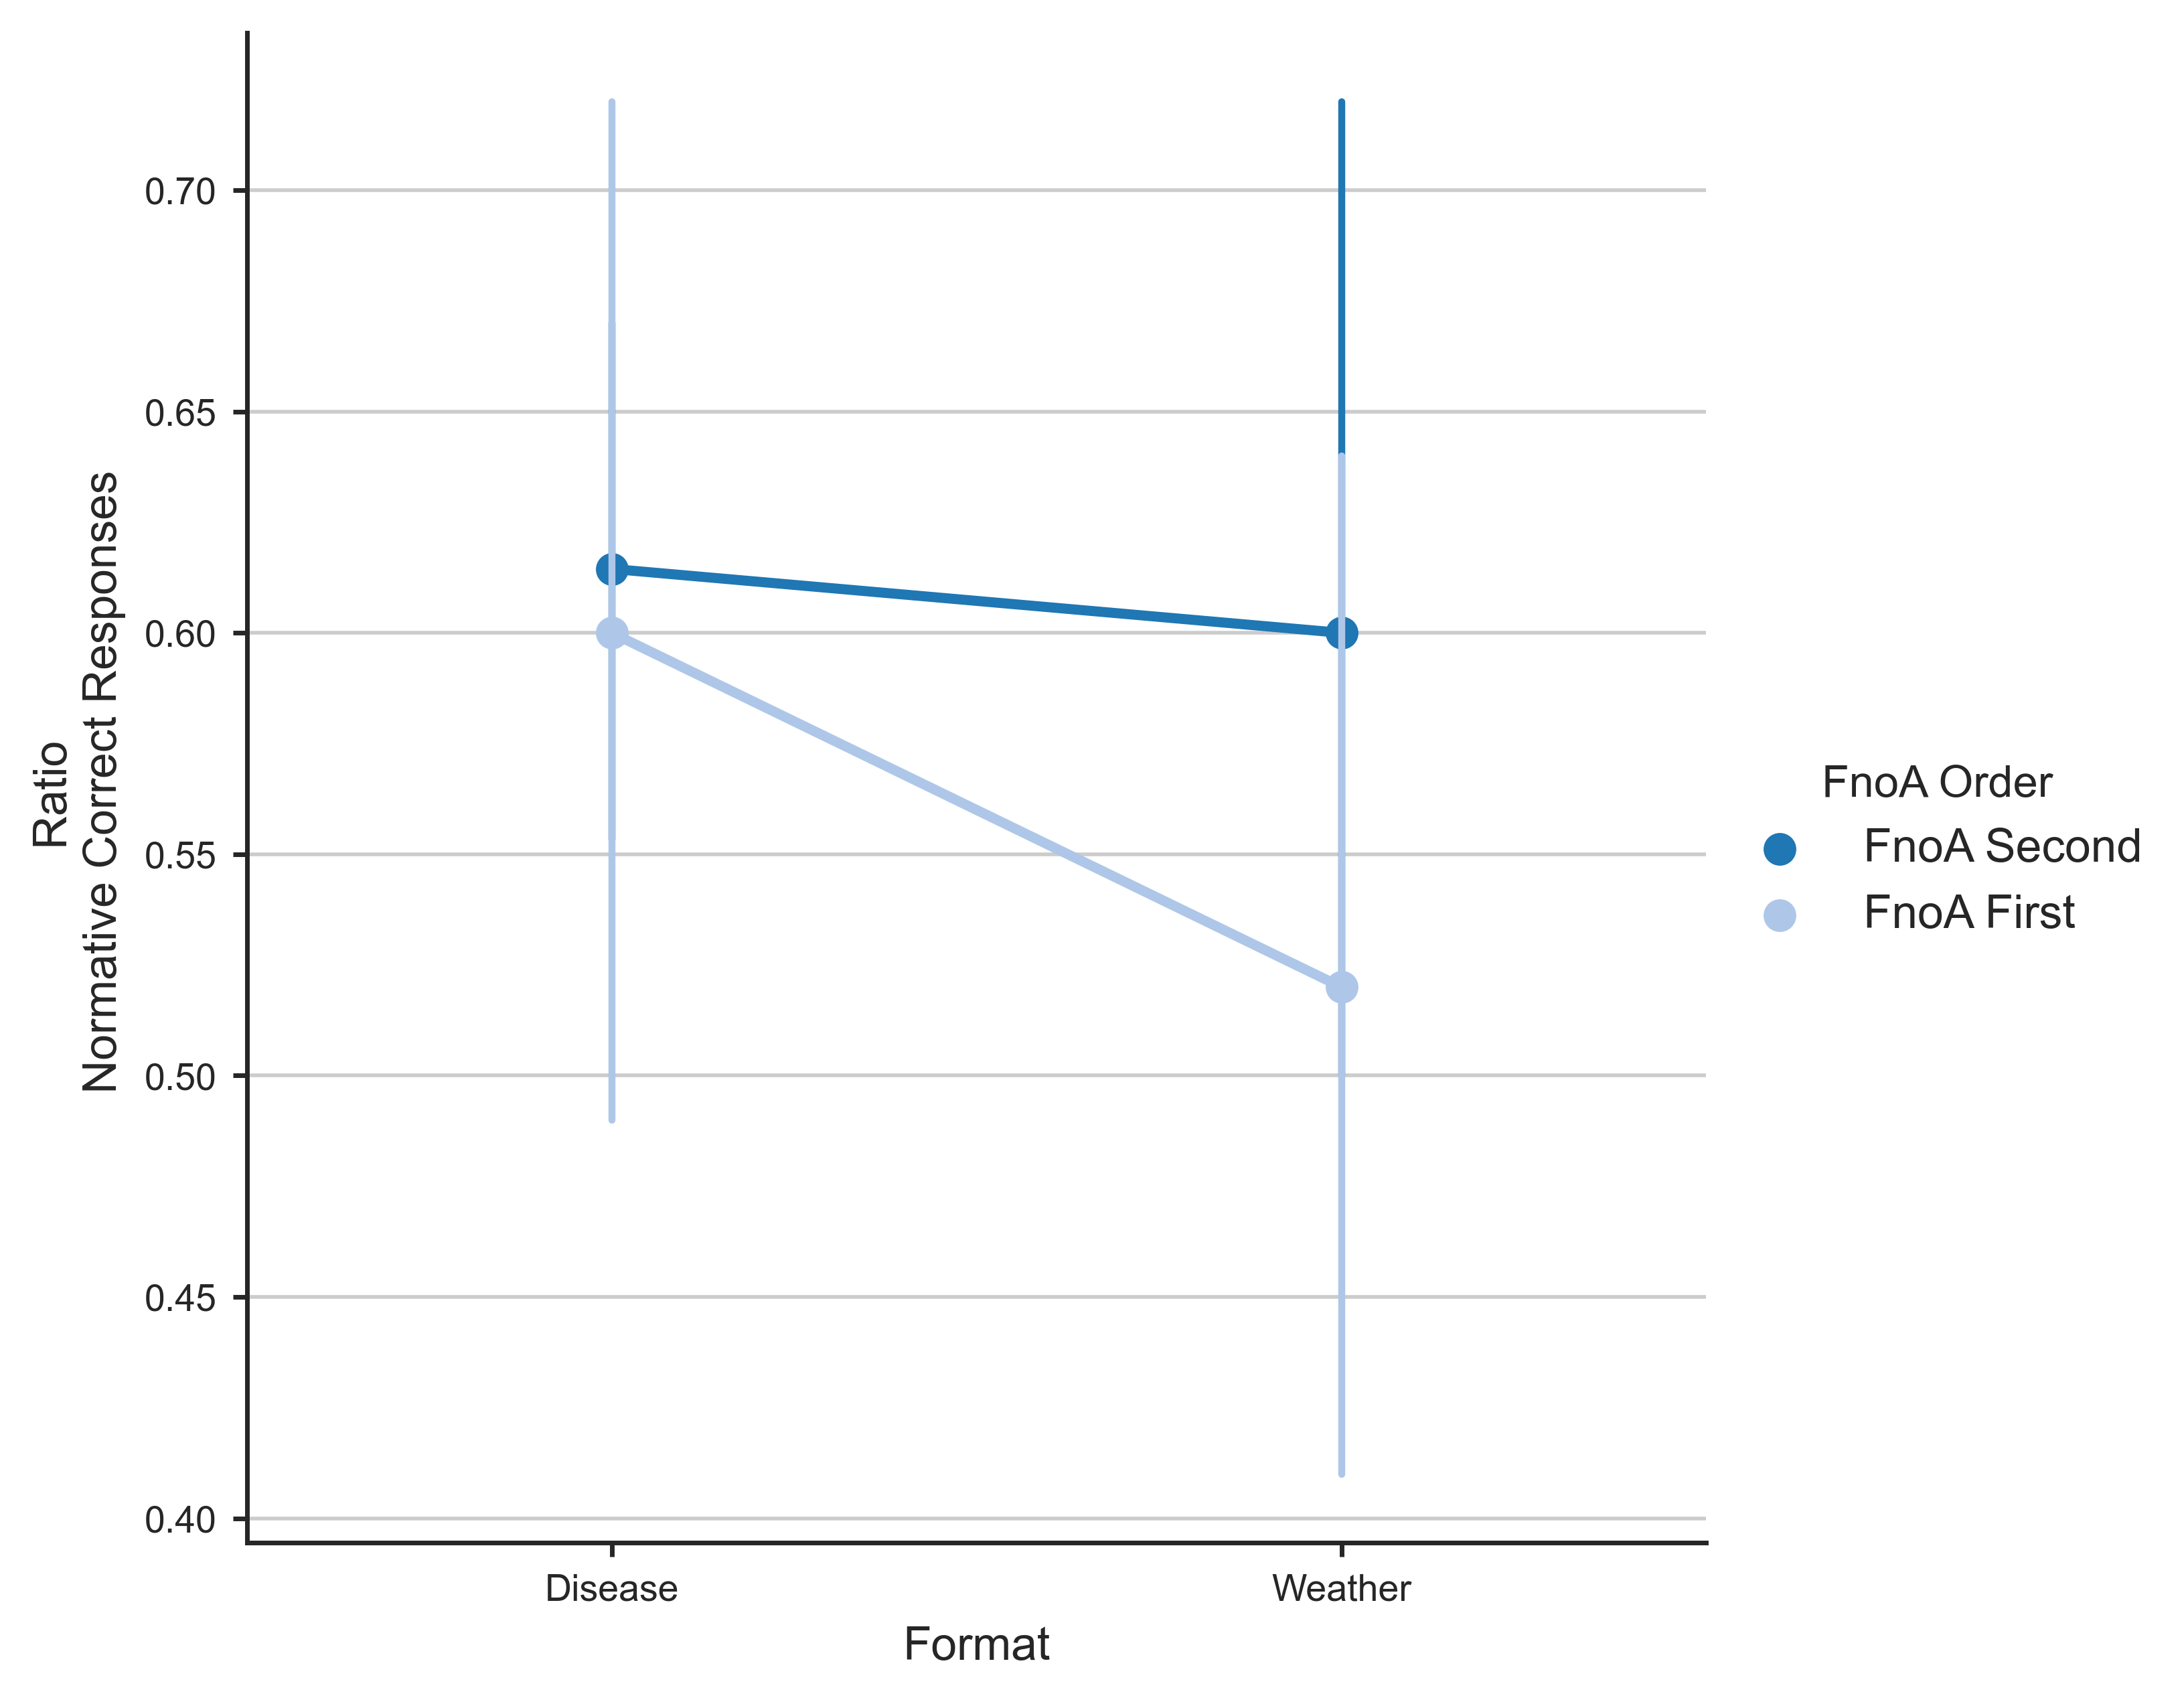
\includegraphics[scale=0.75]{plots/exper_design.png}
    \caption{Effect of the experimental design on the ratio of normatively corrected responses. Dots indicate mean values while vertical bars the relative 95\% confidence interval.}
    \label{factor_plot}
\end{figure}

A binomial regression including the two factors and their interaction was used for explaining variations in the dependent variable and compared with an intercept-only null model as illustarted in \cite{mcelreath2020statistical}. Inspecting the slopes' 95\% Highest Density Interval (HDI) it appears that neither format (-0.217, 0.875), order (-0.232, 0.872) or their interaction (-1.098, 0.460) were able to reliably explain variations in the dependent varibale. This is also supported by the superior performance of the null model as illustrated in figure \ref{deviance_plot}, although the large standard errors suggest caution in assessing the performance of the two models.

\begin{figure}[h!]
    \centering
    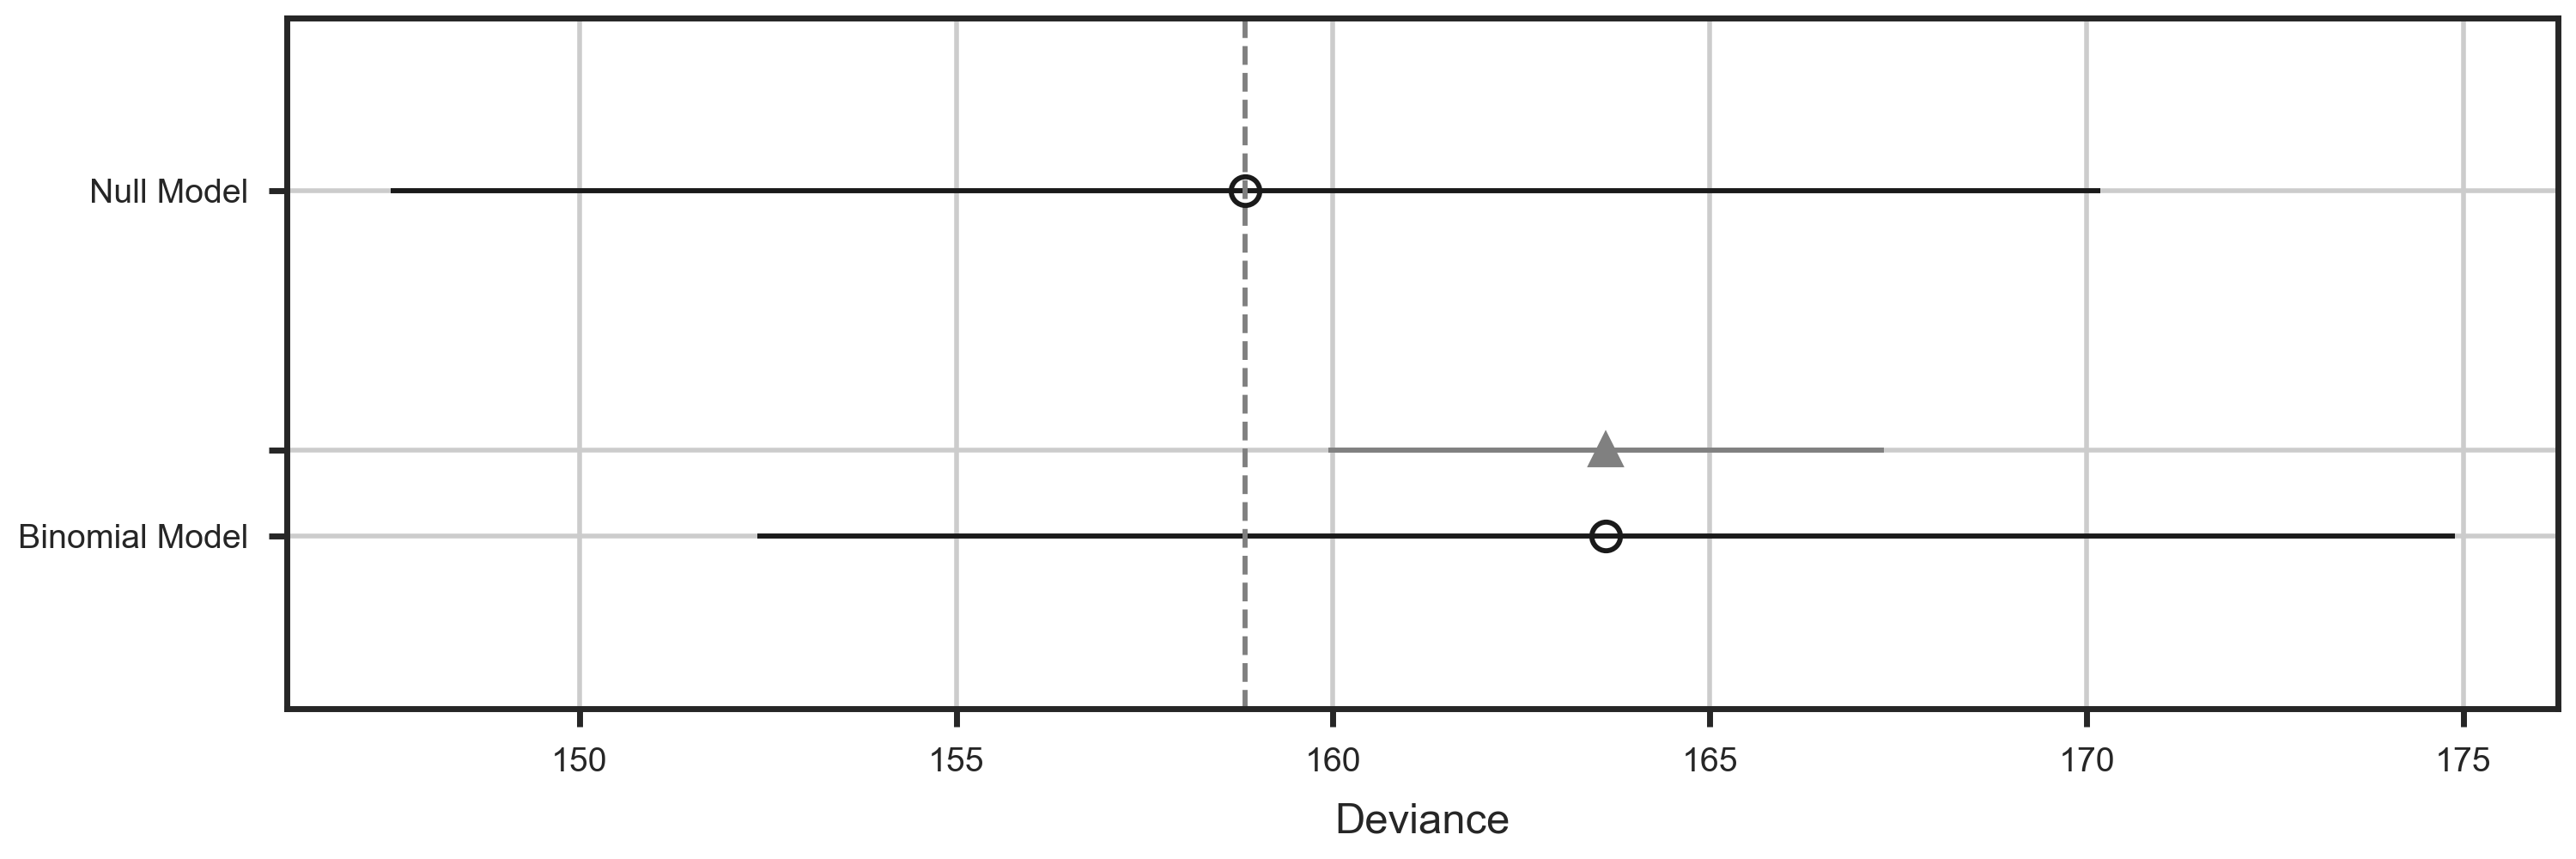
\includegraphics[scale=0.75]{plots/model_comp_deviance.png}
    \caption{Comparison of the binomial model with the null model. The round circles are the out-of-sample mean deviance for a specific score while the black lines indicate the standard deviation. The dotted line indicate the best performing model while the triangle is the difference in Widely-applicable Information Criterion \cite{watanabe2010asymptotic} between the two models with its associated standard error.}
    \label{deviance_plot}
\end{figure}

A correlations analysis, following the example provided in \cite{lee2014bayesian}, was conducted for inspecting the relationship between the dependent variable and a series of covariates. The results can be found in table \ref{Correlation}. As we can see, only for the ian score we can report a reliable although very ephemeral negative correlation with the ratio of normatively correct responses. However, we expect this last one to dissipate if more data are gathered or more restrictive are employed in the data analysis phase.

\begin{table}[h!]
\centering
\caption{Pearson Correlation}
\label{Correlation}
    \begin{tabular}{lrrr}
    \toprule
    Covariate &  Mean Pearson R &  HDI 2.5\% &  HDI 97.5\% \\
    \midrule
          age &       -0.067525 & -0.307789 &   0.168016 \\
           ue &        0.121305 & -0.118642 &   0.356113 \\
           cd &        0.126773 & -0.125257 &   0.372581 \\
          ian &       -0.236972 & -0.470711 &  -0.000884 \\
          inc &        0.100533 & -0.152400 &   0.358970 \\
         epqe &        0.186933 & -0.062156 &   0.438488 \\
         epqp &       -0.007618 & -0.265370 &   0.222962 \\
       bastot &        0.118317 & -0.125261 &   0.354235 \\
        nstot &        0.116159 & -0.145871 &   0.361924 \\
      harmtot &        0.095098 & -0.163266 &   0.339893 \\
    \bottomrule
    \end{tabular}
\end{table}






\printbibliography

\end{document}
